%preamble
\documentclass[letterpaper]{article}
\synctex=1
\usepackage{graphicx}
\graphicspath{ {images/} }

\usepackage{lipsum}
\usepackage{float}
% \bibliographystyle{IEEEtran}
\bibliographystyle{ieeetr}

\usepackage{amssymb}

\usepackage{siunitx}
%actual document
\begin{document}

% \maketitle %insert titlepage here
\begin{titlepage}
 \begin{center}
  \vspace*{1cm}
  \Huge
  Experiment 4
  \vspace{1cm}

  Magnetic Forces
  \vspace{1cm}

  By: Arun Woosaree
  \vspace{1cm}

  Lab partners:
  \vspace{.25cm}
  \Large

  Fatemeh Ghafari Far\\
  % Purvish Jajal
  \vspace{.25cm}
  Yvonne Hong
  \vspace{1cm}

  \Huge
  PHYS 230 Lab EH71
  \vspace{1cm}

  TA: Andrei Tretiakov
  \vspace{1cm}

  Date of Lab: April 5, 2018%\today
  \vfill
 \end{center}
\end{titlepage}

\section{Introduction}
% Begin with experiment’s objectives\\
% Give physical background:\\
% ○ Describe investigated/used\\
% phenomena e.g. Gauss’s law,\\
% field lines, equipotential lines.\\
% ○ Do not copy text from a
% textbook/manual\\
% Provide equations you used\\
% ○ Identify all symbols\\
% \textbf{Equations for this lab}\\
% $$F_z(z)=-\frac{dU}{dz}$$
% $$U=-\mathbf{m}\cdot\mathbf{B}=-\mathbf{mB}\cos{\theta}$$
% $$U=-m_sB_m\cos{\theta}$$
% $$U=-\frac{m_s\mu_0m_m}{2\pi z^3}$$
% $$F_s=\pm \frac{3m_s\mu_0m_m}{2\pi z^4}=\pm\frac{3m_s\mu_0m_m}{2\pi}\frac{1}{z^4}$$
% $$\mathbf{m}=I\mathbf{A}$$
% $$\tao=\mathbf{m}\times\mathbf{B}=mb\sin{\theta}$$
% $$B_z=\frac{\mu_0Ia^2}{2(z^2+a^2)}$$
% \chi

In this experiment, we measure the forces on magnetic material from a strong permanent magnet,
which has an inhomogeneous magnetic field. From the force measurements, we are able to determine the type
of magnetic material. All materials fall into one of three magnetic classes.
Diamagnetic materials are weakly repelled by strong external magnets and paramagnetic materials are weakly attracted
regardless of the direction of the field, and quickly lose any magnetic moment when the external field is removed. Ferromagnetic materials are either `soft' or `hard'. Soft ferromagnets develop
a large net magnetic moment when an external field is applied but like paramagnetic and diamagnetic materials, the moment does not persist if the field is removed.
Hard ferromagnets retain a permanent magnetic dipole moment, even in the absence of an external field. They can be
strongly attracted, repelled and torqued by other magnets, depending on orientation.
We chose to measure the forces of a strong rare earth neodymium magnet (a hard ferromagnet) acting on
another hard ferromagnet, and a soft ferromagnet (a Canadian nickel).

We expect the force-distance power law for the main types of magnetic materials to be in the following format where z is the distance between the materials:
\begin{equation}
 |F_m|=\frac{C}{z^n}, \hspace{1cm}n=4 \hspace{0.1cm} or \hspace{0.1cm} n=7,\hspace{0.5cm} C=some\hspace{0.1cm}constants
\end{equation}
This relation is explored more deeply in the Discussions section.
For hard ferromagnetic samples, an inverse $4^{th}$ power law is predicted $(n=4)$, while for soft ferromagnets, and paramagnetic and diamagnetic materials,
an inverse $7^{th}$ power law is predicted. By analyzing the magnetic force of a strong neodymium magnet on our
samples at various distances, we experimentally confirm that a Canadian nickel is a soft ferromagnetic material, while
a common fridge magnet is a hard ferromagnetic material.

% \textbf{Spicy x: \chi}
\section{Experimental Method}
% List all equipment used\\
% ○ Provide parameters as detailed as
% possible: masses, frequencies,
% etc.\\
% Report what YOU DID to achieve
% experimental goals:\\
% ○ Do not use imperative clause\\
% ○ Use first person narrative or
% passive voice\\
% Based on this section you should be
% able to reproduce your results without a
% manual

%use p1-2 and p2-3 to show setup


\textbf{List of Equipment:}
\begin{itemize}
 \item Milligram-sensitice electronic balance
 \item Strong rare-earth neodymium magnet
 \item Apparatus to hold strong rare-earth magnet at fixed distances
 \item Fridge magnet
 \item Canadian Nickel
 \item 2 red Solo cups
 \item Tape
\end{itemize}

\begin{figure}[H]
 \centering
 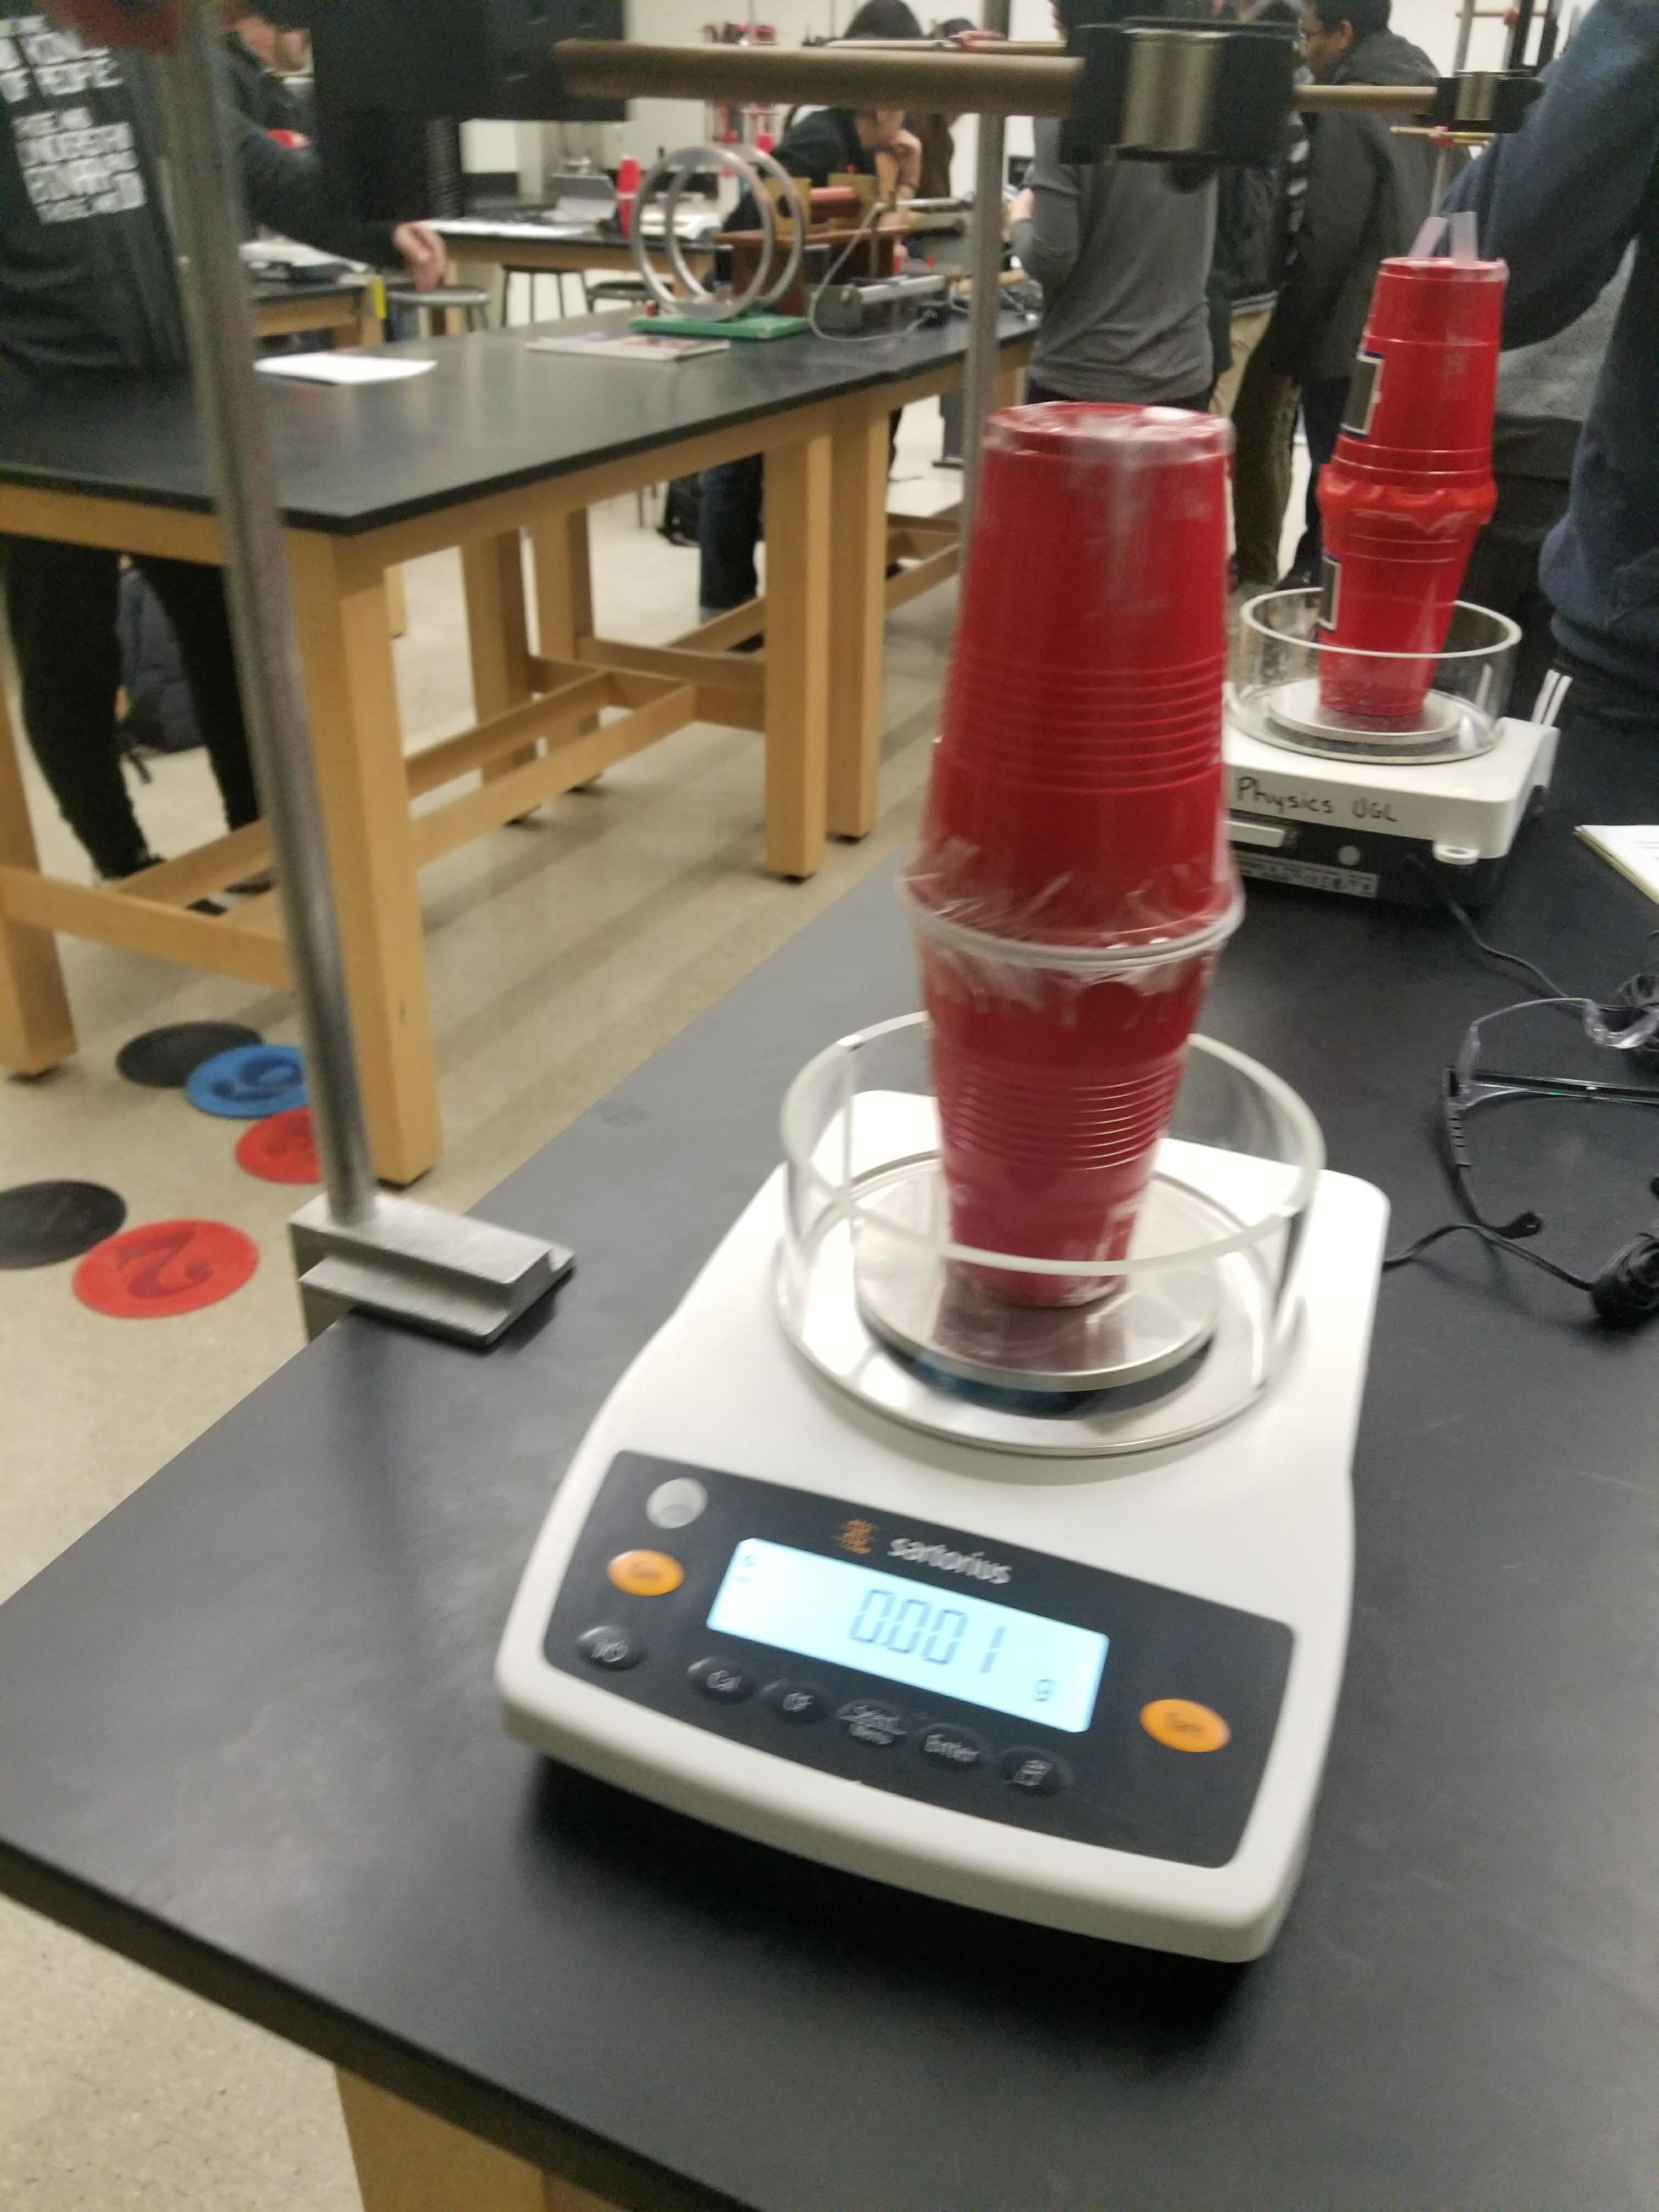
\includegraphics[width=.4\textwidth]{apparatus.jpg}
 \caption{Apparatus used for experiment, along with the electronic balance}
\end{figure}

The experimental setup, as shown in Figure 1 is as follows:
Solo cups taped together are placed on the electronic balance,
and the balance is tared to calibrate its measurement such that
the weight of the cups is not measured. (i.e. only the weight of our
specimens are measured.) For both magnetic materials, an initial reading of the
specimen's weight is taken, which is placed on top of the cups.
The arm is raised as high as possible to keep the strong rare-earth magnet
as far away as possible from the specimen, because at close distances, the reading on the scale
will be skewed, due to the magnetic field of the strong rare-earth magnet.
Then, several measurements are recorded at various distances as the rare-earth magnet is moved towards the
specimen, since the magnetic field of the rare-earth magnet
interacts with the specimen and changes the weight measured by the scale.
The readings on the scale are converted into Newtons, and the distances measured are from the bottom
of the rare-earth magnet to the top of the specimen, measured in metres.


\section{Results}

% \subsection{Part 1}

The raw data recorded for the fridge magnet as a specimen are
as follows:

% Please add the following required packages to your document preamble:
% \usepackage{graphicx}
\begin{table}[H]
 \centering
 \resizebox{\textwidth}{!}{%
  \begin{tabular}{|c|c|c|c|c|}
   \hline
   distance z (m) & balance reading (g) & $|F_m|$ (N)          & $\ln(z)$           & $\ln(|F_m|)$      \\ \hline
   0.494          & 15.863              & 3.92399999999957E-05 & -0.705219761794215 & -10.1458139232672 \\ \hline
   0.347          & 15.87               & 0.00010791           & -1.05843049903528  & -9.1342130115887  \\ \hline
   0.29           & 15.879              & 0.0001962            & -1.23787435600162  & -8.53637601083303 \\ \hline
   0.267          & 15.887              & 0.00027468           & -1.32050662058189  & -8.19990377421178 \\ \hline
   0.249          & 15.896              & 0.00036297           & -1.39030238251743  & -7.92119037174276 \\ \hline
   0.234          & 15.903              & 0.00043164           & -1.45243416362444  & -7.74791865046873 \\ \hline
   0.209          & 15.917              & 0.00056898           & -1.56542102701733  & -7.47166527384059 \\ \hline
   0.199          & 15.931              & 0.00070632           & -1.61445045425764  & -7.25544216537096 \\ \hline
   0.194          & 15.939              & 0.0007848            & -1.63989711991881  & -7.15008164971312 \\ \hline
   0.189          & 15.948              & 0.00087309           & -1.66600826392249  & -7.04347191465486 \\ \hline
   0.184          & 15.953              & 0.00092214           & -1.69281952137315  & -6.988813502117   \\ \hline
   0.179          & 15.963              & 0.00102024           & -1.72036947314138  & -6.88771738524564 \\ \hline
   0.169          & 15.987              & 0.00125568           & -1.77785656405906  & -6.68007802046738 \\ \hline
   0.159          & 16.02               & 0.00157941           & -1.83885107676191  & -6.45070391940254 \\ \hline
   0.154          & 16.038              & 0.00175599           & -1.87080267656851  & -6.34472247854625 \\ \hline
   0.149          & 16.06               & 0.00197181           & -1.90380897303668  & -6.22880337632793 \\ \hline
   0.144          & 16.087              & 0.00223668           & -1.93794197940614  & -6.10276265543256 \\ \hline
   0.139          & 16.116              & 0.00252117           & -1.97328134585145  & -5.98303219949178 \\ \hline
   0.134          & 16.15               & 0.00285471           & -2.00991547903123  & -5.85878501721551 \\ \hline
   0.129          & 16.189              & 0.0032373            & -2.04794287462046  & -5.73301562992648 \\ \hline
   0.124          & 16.243              & 0.00376704           & -2.0874737133771   & -5.58146573179928 \\ \hline
   0.119          & 16.299              & 0.0043164            & -2.12863178587061  & -5.4453335574747  \\ \hline
   0.114          & 16.373              & 0.00504234           & -2.17155683058764  & -5.28988501893184 \\ \hline
   0.109          & 16.453              & 0.00582714           & -2.21640739675299  & -5.14522896502436 \\ \hline
   0.104          & 16.557              & 0.00684738           & -2.26336437984076  & -4.98388918162463 \\ \hline
   0.099          & 16.682              & 0.00807363           & -2.31263542884755  & -4.81915208370993 \\ \hline
   0.098          & 16.708              & 0.00832869           & -2.32278780031156  & -4.78804909807566 \\ \hline
   0.097          & 16.734              & 0.00858375           & -2.33304430047875  & -4.75788439802939 \\ \hline
   0.096          & 16.769              & 0.0089271            & -2.3434070875143   & -4.71866368487611 \\ \hline
   0.095          & 16.8                & 0.00923121           & -2.3538783873816   & -4.68516514480162 \\ \hline
   0.094          & 16.84               & 0.00962361           & -2.36446049671213  & -4.64353582482164 \\ \hline
   0.093          & 16.87               & 0.00991791           & -2.37515578582888  & -4.61341306536653 \\ \hline
   0.092          & 16.904              & 0.01025145           & -2.3859667019331   & -4.58033611998809 \\ \hline
   0.091          & 16.948              & 0.01068309           & -2.39689577246529  & -4.53909316145404 \\ \hline
   0.09           & 16.988              & 0.01107549           & -2.40794560865187  & -4.50302072023734 \\ \hline
   0.089          & 17.038              & 0.01156599           & -2.41911890925     & -4.45968638384963 \\ \hline
   0.088          & 17.071              & 0.01188972           & -2.43041846450393  & -4.43208111775774 \\ \hline
   0.087          & 17.11               & 0.01227231           & -2.44184716032755  & -4.40040977392009 \\ \hline
   0.085          & 17.208              & 0.01323369           & -2.46510402249182  & -4.32498942817925 \\ \hline
   0.082          & 17.372              & 0.01484253           & -2.50103603171788  & -4.21025857059865 \\ \hline
   0.079          & 17.57               & 0.01678491           & -2.53830742651512  & -4.08727501049481 \\ \hline
   0.074          & 17.973              & 0.02073834           & -2.60369018577797  & -3.87577111795682 \\ \hline
   0.064          & 18.888              & 0.02971449           & -2.74887219562247  & -3.51612047335976 \\ \hline
   0.054          & 20.578              & 0.04629339           & -2.91877123241786  & -3.07275609266061 \\ \hline
  \end{tabular}%
 }
 \caption{Measurements of force on the electronic balance with the rare-earth magnet and the fridge magnet at various distances}
\end{table}

\noindent Sample calculation of converting balance reading to force:
\\\rule{10cm}{0.01cm}
\\
balance reading: 15.863g
$$|F_m|=15.863g\times\frac{1kg}{1000g}\times\SI{9.81}{\metre\per\second^2}=\SI{3.92399999999957E-05}{\newton}$$

A linear graph is produced by plotting the natural logarithm of distance from rare-earth magnet to fridge magnet vs. the natural logarithm of the force measured by the balance.
i.e. we plot $\ln(z)$ on the x-axis and $\ln(|F_m|)$ on the y-axis to obtain Figures 2 and 3.
From Equation 1, we can easily see that the slope corresponds to the value -n as follows:
$$|F_m|=\frac{C}{z^n}$$
$$\ln(|F_m|)=\ln\left(\frac{C}{z^n}\right)$$
$$\ln(|F_m|)=-n\ln(z)+ln(C)$$

\begin{figure}[H]
 \centering
 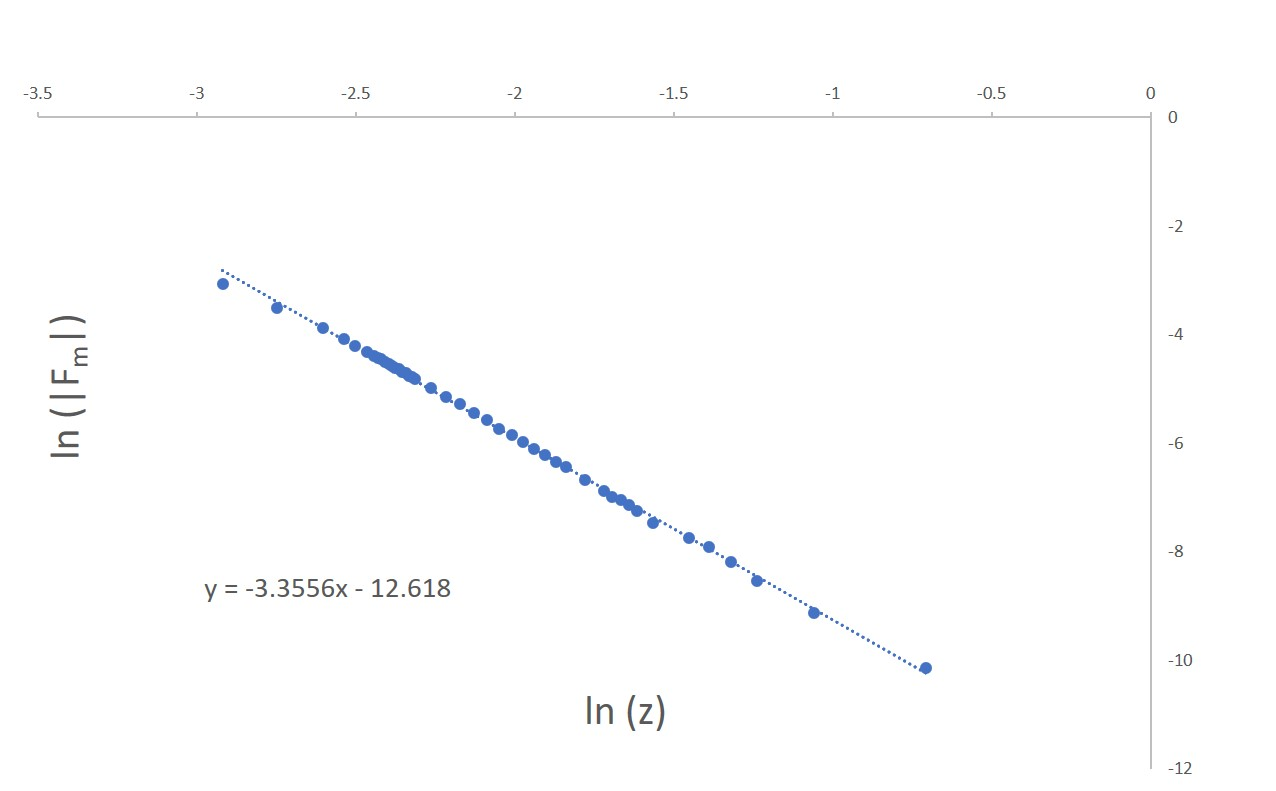
\includegraphics[width=\textwidth]{ferromagnet.jpg}
 \caption{Natural logarithm of distance from rare-earth magnet to fridge magnet vs. natural logarithm of the force measured by the balance }
\end{figure}

\noindent Using Excel's LINEST function, we obtain the following data from the graph in Figure 2:
$$Slope =-3.35557684075733 \pm 0.018881754523524 $$

Thus, we conclude $n=3.36\pm0.02$. Since the fridge magnet is a permanent magnet, it is a hard ferromagnetic material, and n is expected to be 4.
\\ \\
Next, the raw data recorded for the Canadian nickel as the specimen is as follows:
\begin{table}[H]
 \centering
 \resizebox{\textwidth}{!}{%
  \begin{tabular}{|c|c|c|c|c|}
   \hline
   distance z (m) & balance reading (g) & $|F_m|$ (N)           & $\ln(z)$          & $\ln(|F_m|)$      \\ \hline
   0.113          & 3.948               & -3.924E-05            & -10.1458139232671 & -2.1803674602698  \\ \hline
   0.093          & 3.942               & -9.80999999999979E-05 & -9.22952319139298 & -2.37515578582888 \\ \hline
   0.083          & 3.937               & -0.00014715           & -8.82405808328478 & -2.48891467118554 \\ \hline
   0.073          & 3.912               & -0.0003924            & -7.84322883027307 & -2.61729583783375 \\ \hline
   0.063          & 3.857               & -0.00093195           & -6.97823139278646 & -2.7646205525906  \\ \hline
   0.058          & 3.793               & -0.00155979           & -6.46320408216677 & -2.84731226843572 \\ \hline
   0.056          & 3.753               & -0.00195219           & -6.23880345966251 & -2.88240358824699 \\ \hline
   0.055          & 3.731               & -0.00216801           & -6.13394558286925 & -2.90042209374967 \\ \hline
   0.054          & 3.698               & -0.00249174           & -5.99477401736847 & -2.91877123241786 \\ \hline
   0.053          & 3.665               & -0.00281547           & -5.87262606862738 & -2.93746336543002 \\ \hline
   0.052          & 3.635               & -0.00310977           & -5.77320651050972 & -2.95651156040071 \\ \hline
   0.051          & 3.589               & -0.00356103           & -5.63770545012215 & -2.97592964625781 \\ \hline
   0.05           & 3.537               & -0.00407115           & -5.5038297641563  & -2.99573227355399 \\ \hline
   0.049          & 3.486               & -0.00457146           & -5.38792265026136 & -3.01593498087151 \\ \hline
   0.048          & 3.424               & -0.00517968           & -5.26301200068074 & -3.03655426807425 \\ \hline
   0.047          & 3.347               & -0.00593505           & -5.12687982635616 & -3.05760767727208 \\ \hline
   0.046          & 3.268               & -0.00671004           & -5.00415036676445 & -3.07911388249304 \\ \hline
   0.045          & 3.168               & -0.00769104           & -4.86769926403659 & -3.10109278921182 \\ \hline
   0.044          & 3.052               & -0.008829             & -4.72971352106269 & -3.12356564506388 \\ \hline
   0.043          & 2.9                 & -0.01032012           & -4.57365989108935 & -3.14655516328857 \\ \hline
   0.042          & 2.738               & -0.01190934           & -4.43043231276756 & -3.17008566069877 \\ \hline
   0.041          & 2.547               & -0.01378305           & -4.28431570261916 & -3.19418321227783 \\ \hline
   0.04           & 2.312               & -0.0160884            & -4.12965676356876 & -3.2188758248682  \\ \hline
   0.039          & 2.042               & -0.0187371            & -3.97724976334633 & -3.24419363285249 \\ \hline
   0.038          & 1.726               & -0.02183706           & -3.82414675255151 & -3.27016911925575 \\ \hline
   0.037          & 1.349               & -0.02553543           & -3.66768837939244 & -3.29683736633791 \\ \hline
   0.036          & 0.86                & -0.03033252           & -3.49553487467969 & -3.32423634052603 \\ \hline
   0.035          & 0.237               & -0.03644415           & -3.31197432723514 & -3.35240721749272 \\ \hline
  \end{tabular}
 }
 \caption{Measurements of force on the electronic balance with the rare-earth magnet and the Canadian nickel at various distances}
\end{table}
The graph is also produced in the exact same way as before with the fridge magnet specimen:
\begin{figure}[H]
 \centering
 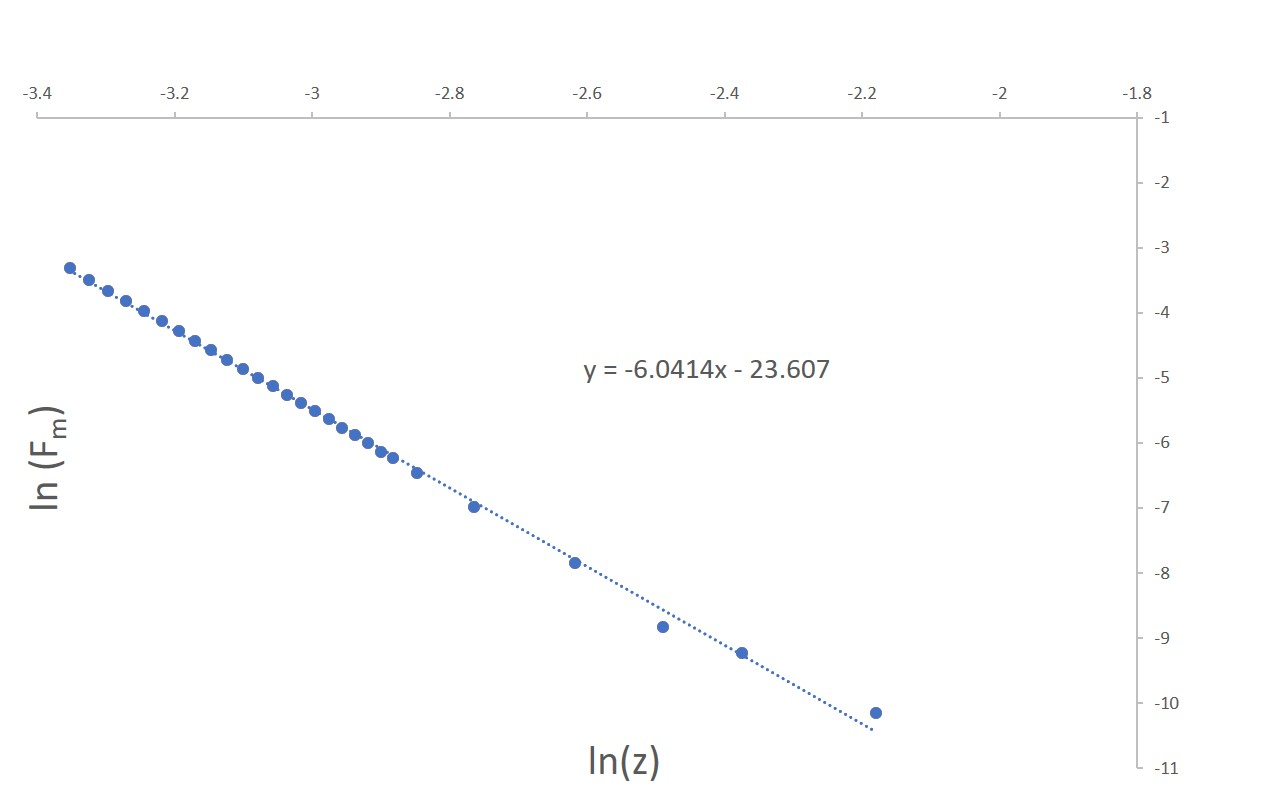
\includegraphics[width=\textwidth]{nickel.jpg}
 \caption{Natural logarithm of distance from rare-earth magnet to Canadian nickel vs. natural logarithm of the force measured by the balance }
\end{figure}
\noindent Using Excel's LINEST function, we obtain the following data from the graph in Figure 3:
$$Slope =-6.04142520404573 \pm 0.055033493756539 $$

Thus, we conclude $n=6.04\pm0.06$. Since the nickel does not produce its own magnetic field, but is strongly attracted to hard ferromagnetic material, it is a soft ferromagnetic material, and n is expected to be 7.


% \\ \\
% \subsection{Part 2}
%
% The raw data recorded for part 2 where we beasure $B_H$ in the
% Helmholtz coils as a function of current is outlined in Table 2.
%
% \begin{table}[H]
%  \centering
%  \begin{tabular}{|c|c|}
%   \hline
%   Current (A) & $B_H (T)$          \\ \hline
%   0.1         & -0.000194861519119 \\ \hline
%   0.2         & -0.000133962572081 \\ \hline
%   0.3         & -6.99808991888E-05 \\ \hline
%   0.4         & -1.21344552038E-05 \\ \hline
%   0.5         & 4.36568382113E-05  \\ \hline
%   0.6         & 0.000108031407536  \\ \hline
%   0.7         & 0.000168628126549  \\ \hline
%   0.8         & 0.000230010638426  \\ \hline
%   0.9         & 0.000286799284324  \\ \hline
%   1           & 0.000351052962439  \\ \hline
%  \end{tabular}
%  \caption{Measured magnitudes of $B_H$ when varying the current in the coil in 0.1A increments}
% \end{table}
%
% Given that $R=14.8 \pm 0.2 cm$, we can linearize Equation 3 to
% generate a graph (Figure 5), from which we can determine the experimental
% value for N  as follows:
%
% $$ B_H = \frac{8\mu_0NI}{\sqrt{125}R} \Rightarrow B_H = N\left( \frac{8\mu_0I}{\sqrt{125}R} \right)  $$
% % $$ \therefore B_H = \frac{8 \times \SI{4 \pi e-7}{\tesla\metre\per\ampere}}{\sqrt{125}(\SI{14.8}{\cm})}$$
% % $$ \Rightarrow N = \frac{B_H \sqrt{125} R}{8\mu_0I} $$
% % $$ \therefore N= \frac{}{} $$
% %  so we generate a graph
% % with $\frac{\sqrt{2V}}{r}$ on the X axis using our measured voltage values, and $B_H$ on the Y axis
% % using our measured current values.
% Using the form above, we can plot a graph, such that
% $B_H$ is on the y-axis, and $\frac{8\mu_0NI}{\sqrt{125}R}$ is plotted on the x-axis.
% Then, our experimental value for N will be the slope, and the y-intercept should theoretically be zero.
% \begin{figure}[H]
%  \centering
%  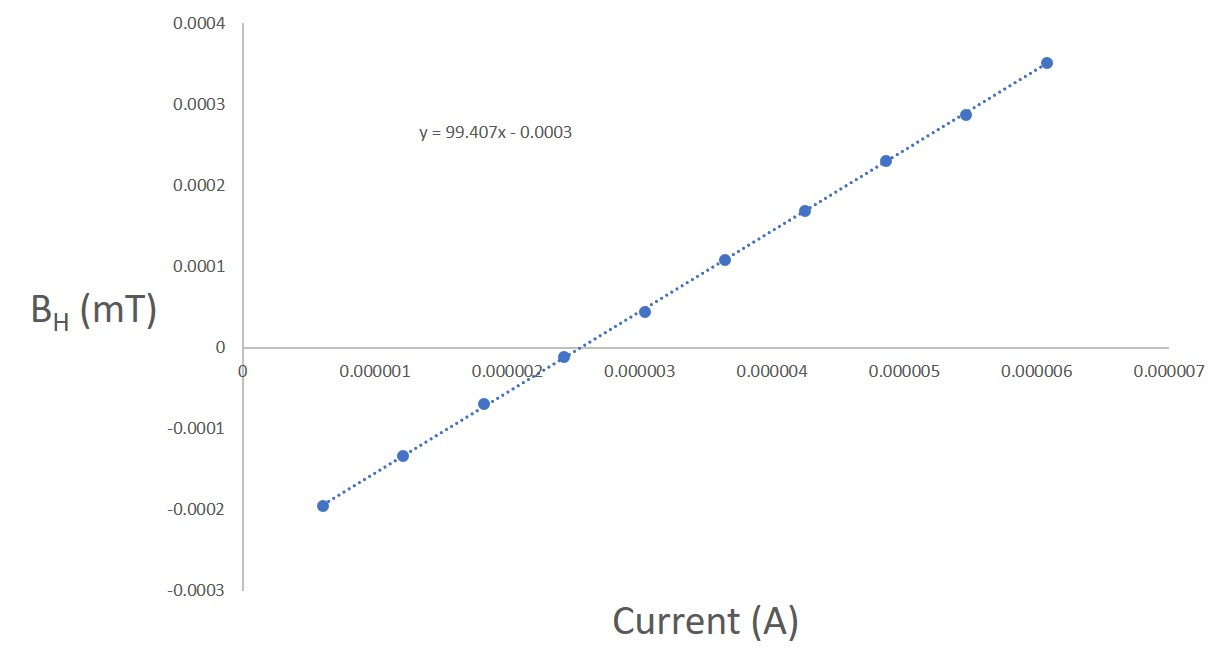
\includegraphics[width=\textwidth]{p2graph.jpg}
%  \caption{$B_H$ as a function of current}
% \end{figure}
%
% \newpage
% \noindent Using Excel's LINEST function, we obtain the following data from the graph in Figure 5.
% \begin{table}[H]
%  \centering
%  \begin{tabular}{cc}
%   Slope & $=99.4073706 \pm 0.3873961 $ \\
%         & $=99.4 \pm 0.4$
%   % Y-Intercept: &  $\num{3.99642631798173E-05}\pm \num{6.40167504007098E-06}$ \\
%  \end{tabular}
%  % \caption{LINEST data from the graph in Figure 3}
% \end{table}
%
% Now, our slope corresponds to N, however to determine our experimental
% value for N, we use the scaling factor $\frac{B_t}{B_{exp}}=1.33$ which was
% determined in Part 1 of the experiment.
%
% $$ N= 99.4 \times 1.33 \approx 132 \:turns $$
% $$ \delta N   = 0.4 \times 1.33 \approx 1 $$
% $$ \therefore N = 132 \pm 1 \:turns$$
% The theoretical $N=133$
%
% % \vspace{1cm}
% % \noindent The calculated values of $e/m$ and $B_E$ from the graph are summarized in Table 3.
% % \begin{table}[H]
% % \centering
% % \begin{tabular}{c|c|c|c|}
% %                 & Expected                      & Calculated:                                     & \% Error \\ \hline
% % $e/m$: & $\SI{1.76e11}{\coulomb\per\kilogram}$      & $\num{1.70e11} \pm \SI{4.91e9}{\coulomb\per\kilogram}$  &    $3.52$  \\ \hline
% % $B_E$: & $4.8 \pm \,\SI{0.3e-5}{\tesla}$           & $\num{4.00e-5} \pm \,\SI{6.40e-6}{\tesla}$                    &   $16.74$  \\ \hline
% % \end{tabular}
% % \caption{Measured values of $e/m$ and $B_E$ compared to the calculated values obtained from the graph.}
% % \end{table}

\section{Discussion}

From our results, we were able to clearly classify the magnetic materials as either soft ferromagnetic or hard ferromagnetic.
With experimentally determined values of $3.36\pm0.02$ for the fridge magnet, and $6.04\pm0.06$ for n in Equation 1, we
clearly see that the inverse power law relation for the magnetic force as a function of distance acting on the Canadian nickel falls off quite faster
than the magnetic force on the fridge magnet. This implies that the nickel is the soft ferromagnetic material, while the permanent fridge magnet is the
hard ferromagnetic material. However, our experimentally determined results do not agree within error of the expected values.
For hard ferromagnetic samples, an inverse $4^{th}$ power law is expected, while for soft ferromagnets, is expected.
Although our results did not agree within error of the expected values,
the graphs both fit linear curves, with no noticeable anomalous data points relative to the trendlines.
This implies the source of error was constant, which can likely be attributed to a combination of the following:
While attempting to measure the weights on the balance, the readings fluctuated which made it difficult to
measure accurately. It is also likely that human error was introduced from measuring the distances, and/or
not having the strong rare-earth magnet's center directly align with the magnetic specimens' centres even though
we tried to minimize these sources of error.

As mentioned before, in Equation 1, C is a bunch of constants, and z is raised to the power of either 4 or 7 depending
on the type of magnetic material.
For hard ferromagnetic materials, Equation 1 is more completely represented by:
\begin{equation}
 F_z=\pm\frac{3m_s\mu_0m_m}{2\pi}\frac{1}{z^4}
\end{equation}
,where $m_s$ is the dipole moment on the sample hard ferromagnet, $\mu_0=\SI{4\pi e-7}{\henry\per\metre}$ is the magnetic permeability
of free space, $m_m$ is the dipole moment from the strong rare-earth magnet, and z is the distance between the two magnets, in metres.

For soft ferromagnetic materials, and paramagnetic and diamagnetic materials, Equation 1 is more
completely represented by:
\begin{equation}
 F_z=\frac{3\mu_0\chi Vm_m}{2\pi^2}\frac{1}{z^7}
\end{equation}
,where V is the volume, and $\chi$ is the magnetic susceptibility of the sample material.
% Equation 2 can be derived with the knowledge that $$F_z(z)=-\frac{dU}{dz}$$,
% where U is the potential energy. Also, U can be expressed in terms of a magnetic
% moment \textbf{m} and magnetic field \textbf{B}:
% $$U-\mathbf{m}\cdot\mathbf{B}$$
% Thus, U can be written as:
% $$U=-\frac{m_s\mu_0m_m}{2\pi z^3}$$
\\ \\ \textbf{The sign of $\chi$}:\\
To obtain our graphs in Figures 2 and 3, Equation 1 was linearized to obtain:
$$\ln(|F_m|)=-n\ln(z)+ln(C)$$
The magnetic susceptibility $\chi$ is positive or negative, depending on the
%non-ferromagnetic
material,
%(i.e. paramagnetic or diamagnetic)
which determines if the magnetic force is attractive or repulsive.
For by observing the equation our graph is based on above, C had to be positive, or it would have been impossible to
obtain the natural logarithm $\ln(C)$.
Therefore, in Equation 3, $\chi$ must be positive, in order for C to be positive.
% For the fridge magnet, which was set up so that it repelled, $\chi$ would then be negative, by the
% definition above, and since the nickel experienced an attractive force from the strong neodymium magnet,
% $\chi$ for the nickel would be positive.
This is further reinforced by the observation that the magnetic force is attractive when the
strong magnet gets close to the nickel, as the nickel would stick to the rare-earth magnet very strongly if the magnet got too close.%, which is a soft ferromagnetic material and therefore has the inverse $7^{th}$ power
% relation expressed in Equation 3.


% \subsection{Part 1}
%
% The right hand rule is used to determine the
% direction of the magnetic $\textbf{B}$ field in the coils of wire. In the case of the
% solenoid, the magnetic field is illustrated in Figure 5 below:
%
% % \begin{figure}[H]
% %  \centering
% %  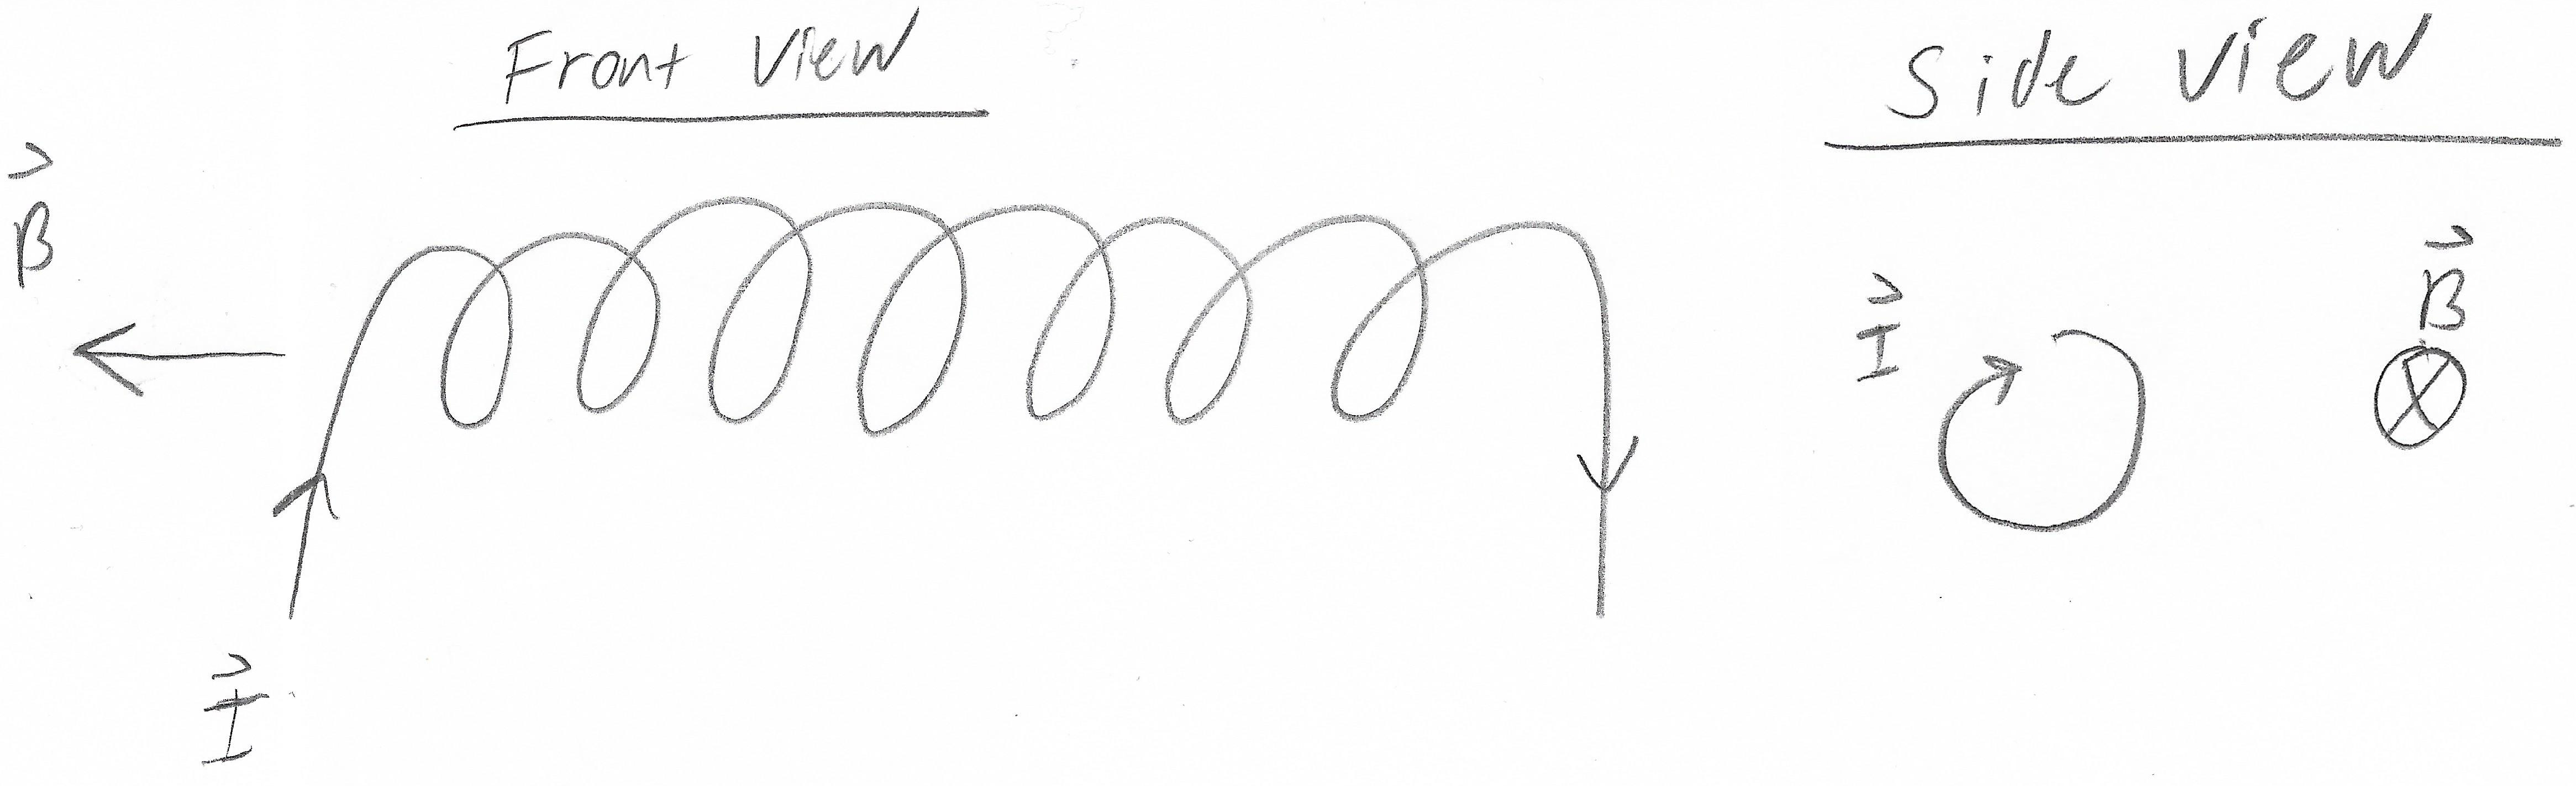
\includegraphics[width=\textwidth]{question1.jpg}
% %  \caption{Orientation of \textbf{B} vector for a solenoid with current \textbf{I} running through it.}
% % \end{figure}
%
% From Figure 4, we can see that the experimental values measured are quite different
% compared to the theoretical values. However, the shape of both curves are very similar.
% In fact, if the experimental values were offset by a scaling factor $\frac{B_t}{B_{exp}}=1.33$ , our
% measured results would be extremely close to the expected theoretical curve. Therefore,
% the cause of error is constant, which implies that the Hall probe is likely miscalibrated,
% or it could be a result of our equations not taking into account the internal resistance of the wires.
%
%
%
% \subsection{Part 2}
%
%
% The graph produced (Figure 5) is linear as expected, with no anomalous data points.
% Using the scaling factor 1.33 derived in part 1 of the experiment, we obtain the value $N=132 \pm 1$,
% from the slope of the graph in Figure 5, which agrees within error of the theoretical value 133.
%
% % \begin{figure}[H]
% %   \centering
% %   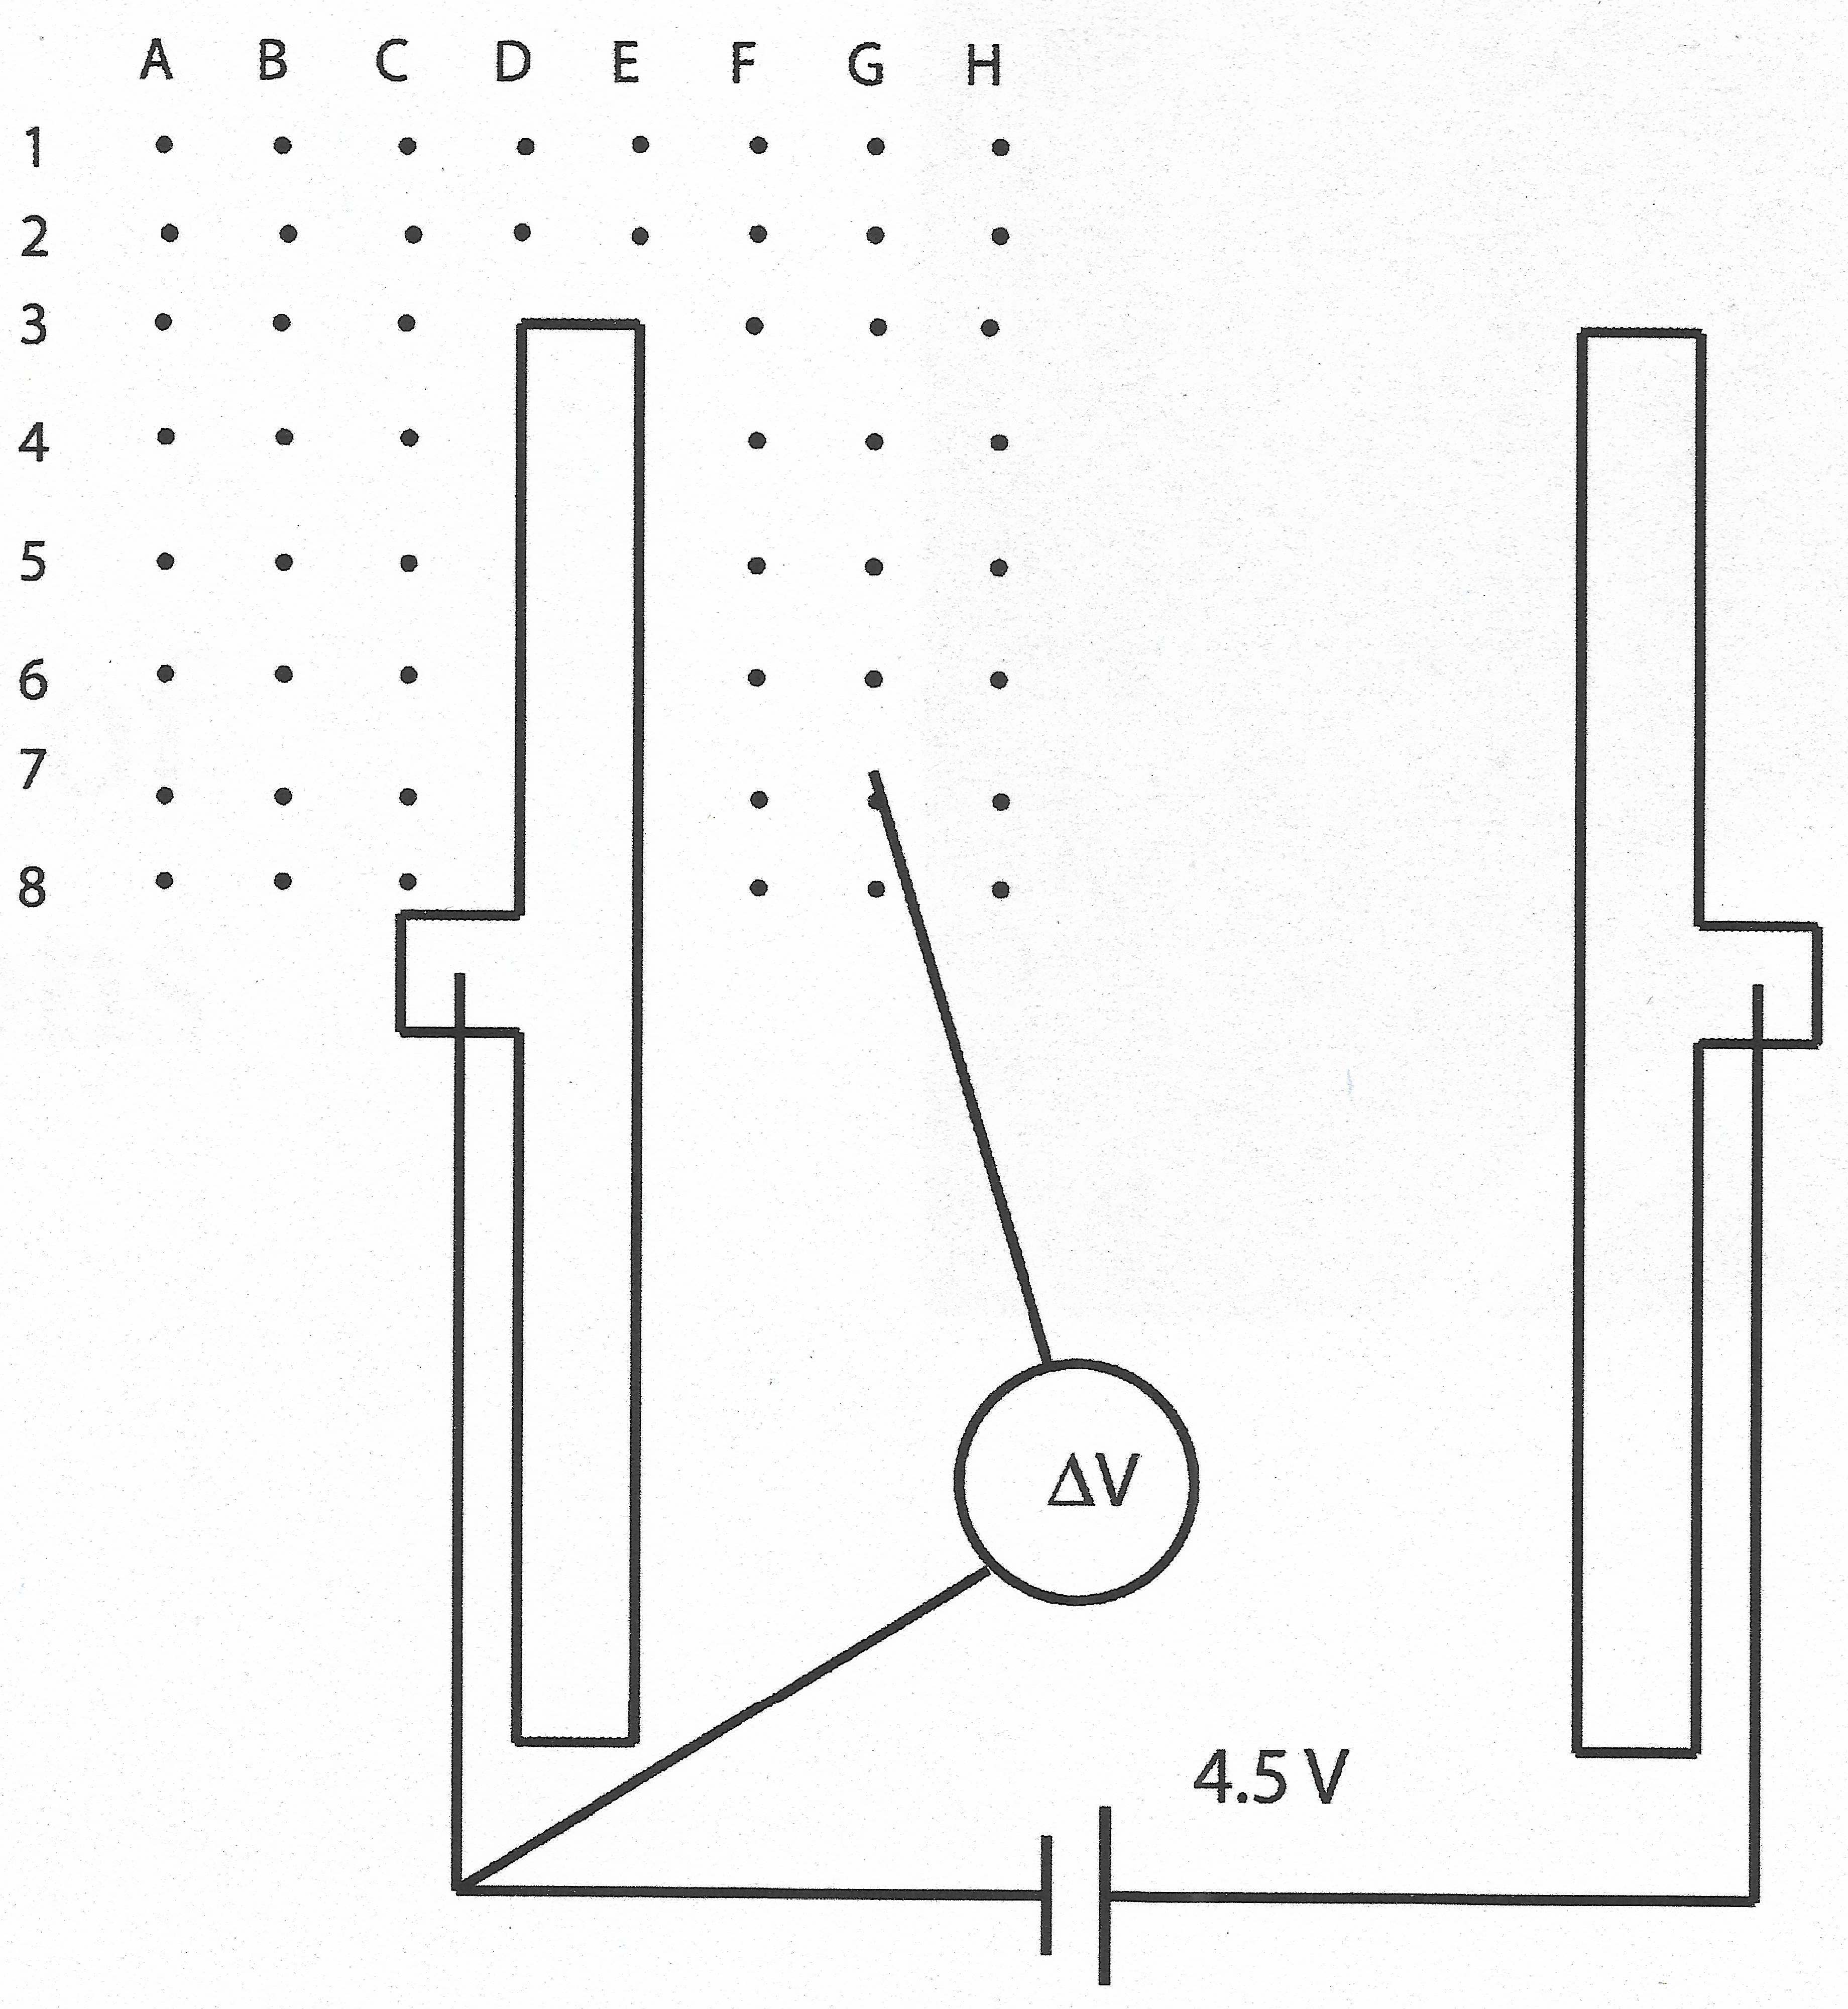
\includegraphics[width=\textwidth]{fig3.jpg}
% %   \caption{The direction of the \textbf{B} field is found to be pointing out of the page when drawn this way.}
% % \end{figure}
%
% % SOME MORE DERIVATIONS AS FOLLOWS:
%
% Using equation 1, and the geometry from Figure 1, we can find a simplified expression for $B_s$ in the centre of a real solenoid as follows:
% $$ \cos{\beta_2} = \frac{L/2}{\sqrt{R^2+L^2/4}}$$
% $$ \cos{\beta_1} = \sin{(\pi/2 - \beta_1)} = -\sin{(\beta_1-\pi/2)} = -\frac{L/2}{\sqrt{R^2+L^2/4}}  $$
% Substituting into equation 1 yields:
% $$ B_s = 1/2 \mu_0nI \left(\frac{L/2}{\sqrt{R^2+\frac{L^2}{4}}} + \frac{L/2}{\sqrt{R^2+\frac{L^2}{4}}} \right) =  1/2\mu_0nI \left(\frac{L}{\sqrt{R^2+\frac{L^2}{4}}} \right)= \frac{\mu_0nIL}{\sqrt{4R^2+L^2}}$$
% Since $n=N/L$, we can substitute $nL=N$ to finally obtain:
% $$ B_s= \frac{\mu_0NI}{\sqrt{4R^2+L^2}} $$
% %and compare it to the
% %expected value of 133. The radius of each coil is $14.8\pm 0.2cm$
%
% We can also find an expression for $B_c$ in the centre of a single coil using Equation 2 as follows:\\
% At the centre of the coil, $x=x_c$ to obtain:
% $$ B_c = \frac{\frac{1}{2} \mu_0NR^2I}{(R^2+(x_c-x_c)^2)^{3/2}} $$
% which simplifies nicely:
% $$ \frac{\frac{1}{2} \mu_0NR^2I}{(R^2)^{3/2}} = \frac{\frac{1}{2} \mu_0NR^2I}{R^3}  $$
% $$ \therefore B_c = \frac{\frac{1}{2} \mu_0NI}{2R} $$
%
% Additionally, the expression for $B_H$ can be obtained from the expression for $B_c$ derived above. By inspection,
% we notice that $x-x_c=R/2$, which we can substitute into Equation 2 to obtain:
% $$ B_c= \frac{\frac{1}{2}\mu_0NR^2I}{(R^2+(\frac{R}{2})^2)^{3/2}} = \frac{\frac{1}{2}\mu_0NR^2I}{\frac{\sqrt{125}}{8}R^3} = \frac{1}{2}\times \frac{8\mu_0NI}{\sqrt{125}R} $$
% and by realizing that $2B_c=B_H$, we finally obtain Equation 3 by multiplying the above expression by 2:
% $$B_H=\frac{8\mu_0NI}{\sqrt{125}R}$$


\section{Conclusions}
In Experiment 4, we measure the forces on magnetic material from a strong permanent magnet at varying distances.
From the force measurements, we were able to classify the type
of magnetic material (soft or hard ferromagnetic). The specimens were a fridge magnet, and a Canadian nickel, which are
a hard ferromagnetic material and soft ferromagnetic material, respectively.
The force-distance relation for the fridge magnet was expected to have an inverse $4^{th}$ power law, and the experimentally obtained
value was $3.36\pm0.02$.
An inverse $7^{th}$ power law was expected for the nickel, and the experimentally obtained value was $6.04\pm0.06$.
While the values do not agree within error, it is easy to see that the soft ferromagnetic material (the nickel) had a inverse power law
falloff significantly faster than the hard ferromagnetic material (the fridge magnet), which is what was expected of the experiment.
Errors in the experimentally determined value can be attributed to the electronic balance's measurements fluctuating, and
human error in measuring the distances. Overall, the graphs fit the linear trend that was expected, and while the
results do not agree within error, we were still able to classify the magnetic materials correctly.


% \bibliography{references}
\end{document}
